\subsubsection{Scattering of Scalar Nucleons}
Let's go back to the scalar Yukawa theory of the section \ref{sec:ScYukawa} and 
consider nucleon scattering process $\psi \psi \to \psi \psi$.
\begin{eqnarray}
\begin{array}{l}
\ketend i \ket
=
b^\dagger(\bld{p}_a) b^\dagger(\bld{p}_b) \ketend 0 \ket
\rightdef
\ketend N_a N_b \ket
\\
\ketend f \ket
=
b^\dagger(\bld{p}_1) b^\dagger(\bld{p}_2) \ketend 0 \ket
\rightdef
\ketend N_1 N_2 \ket
\end{array}
\end{eqnarray}
The first contribution to $S - 1$ in Eq. (\ref{eqn:SmatrixPertSer}) arise from 
the second order term in $H_I$. It reads
\begin{eqnarray}
\bra f \braend S - 1 \ketend i \ket
&\stackrel{(2)}{=}&
\frac{(-i g)^2}{2} \int d^4 x_1 d^4 x_2
\bra f \braend
T[
\normalprod{\psi^\dagger(x_1) \psi(x_1) \phi(x_1)}
\nonumber\\
&&
\hspace{35mm}
\times
\normalprod{\psi^\dagger(x_2) \psi(x_2) \phi(x_2)}
]
\ketend i \ket
\nonumber\\
&=&
\frac{(-i g)^2}{2} \int d^4 x_1 d^4 x_2
\Delta_F(x_1 - x_2)
\nonumber\\
&&
\hspace{12mm}
\bra N_2 N_1 \braend
\normalprod{
\psi^\dagger(x_1) \psi(x_1) 
\psi^\dagger(x_2) \psi(x_2)
}
\ketend N_a N_b \ket\,,
\nonumber\\
\label{eqn:scYS2ndord}
\end{eqnarray}
%-------------------------------------------
The sandwich $\bra N_2 N_1 \braend \dots \ketend N_a N_b \ket$ reads
\begin{eqnarray}
&&\bra N_2 N_1 \braend
\normalprod{
\psi^\dagger(x_1) \psi(x_1) 
\psi^\dagger(x_2) \psi(x_2)
}
\ketend N_a N_b \ket
\nonumber\\
&=&
\int \frac{d^3 \bld{p}_1' d^3 \bld{p}_2'}{(2\pi)^3 4 {p_1^0}' {p_2^0}'} 
 \frac{d^3 \bld{p}_a' d^3 \bld{p}_b'}{(2\pi)^3 4 {p_a^0}' {p_b^0}'} 
 e^{i(p_1' x_1 + p_2' x_2 - p_a' x_1 - p_b' x_2)}
\nonumber\\
&&
 \bra 0 \braend 
 b(\bld{p}_2)  b(\bld{p}_1) \left\{
 b^\dagger(\bld{p}_1') b^\dagger(\bld{p}_2')
b(\bld{p}_a') b(\bld{p}_b')
\right\}
 b^\dagger(\bld{p}_a) b^\dagger(\bld{p}_b)
 \ketend 0 \ket
\nonumber\\
&=&
\int \frac{d^3 \bld{p}_1' d^3 \bld{p}_2'}{(2\pi)^3 4 {p_1^0}' {p_2^0}'} 
 \frac{d^3 \bld{p}_a' d^3 \bld{p}_b'}{(2\pi)^3 4 {p_a^0}' {p_b^0}'} 
 e^{i(p_1' x_1 + p_2' x_2 - p_a' x_1 - p_b' x_2)}
\nonumber\\
&&
\bra 0 \braend 
 b(\bld{p}_2)  \left\{
 2{p_1^0}' \delta^3(\bld{p}_1' - \bld{p}_1) 
 + b^\dagger({\bld{p}_1'}) b({\bld{p}_1})
 \right\}
 b^\dagger({\bld{p}_2'})
 \nonumber\\
 &&
  b(\bld{p}_a')   \left\{
 2{p_b^0}' \delta^3(\bld{p}_b' - \bld{p}_b) 
 + b^\dagger({\bld{p}_b}) b({\bld{p}_b'})
  \right\}
  b^\dagger({\bld{p}_a})
   \ketend 0 \ket
\nonumber\\
&=&
\int \frac{d^3 \bld{p}_1' d^3 \bld{p}_2'}{(2\pi)^3 4 {p_1^0}' {p_2^0}'} 
 \frac{d^3 \bld{p}_a' d^3 \bld{p}_b'}{(2\pi)^3 4 {p_a^0}' {p_b^0}'} 
 e^{i(p_1' x_1 + p_2' x_2 - p_a' x_1 - p_b' x_2)}
\nonumber\\
&&
\bra 0 \braend 
\left\{
4{p_1^0}' {p_2^0}' \delta^3(\bld{p}_1' - \bld{p}_1) \delta^3(\bld{p}_2' - \bld{p}_2) 
+
4{p_2^0}' {p_1^0}' \delta^3(\bld{p}_1' - \bld{p}_2) \delta^3(\bld{p}_2' - \bld{p}_1) 
\right\}
\nonumber\\
&&
\left\{
4{p_a^0}' {p_b^0}' \delta^3(\bld{p}_a' - \bld{p}_a) \delta^3(\bld{p}_b' - \bld{p}_b) 
+
4{p_a^0}' {p_b^0}' \delta^3(\bld{p}_a' - \bld{p}_b) \delta^3(\bld{p}_b' - \bld{p}_a) 
\right\}
\ketend 0 \ket
\nonumber\\
&=&
\frac{1}{(2\pi)^6}
\left\{
e^{i(p_1 x_1 + p_2 x_2)} + e^{i(p_2 x_1 + p_1 x_2)}
\right\}
\left\{
e^{-i(p_a x_1 + p_b x_2)} + e^{-i(p_b x_1 + p_a x_2)}
\right\}
\nonumber
\end{eqnarray}
Substituting this result and adopting the expression (\ref{eqn:scFeynmanProp})
in Eq. (\ref{eqn:scYS2ndord}),
we obtain
\begin{eqnarray}
\bra f \braend S - 1 \ketend i \ket
&=&
\frac{(-i g)^2}{2 (2\pi)^6} \int \frac{d^4 k}{(2\pi)^4} 
\frac{i}{k^2 - m^2 + i\epsilon}
\int d^4 x_1 d^4 x_2
\left\{
e^{i(p_1 + k - p_a)x_1}e^{i(p_2 - k - p_b)}
\right.
\nonumber\\
&&
+
e^{i(p_2 + k - p_a)x_1}e^{i(p_1 - k - p_b)}
+
e^{i(p_1 + k - p_b)x_1}e^{i(p_2 - k - p_1)}
\nonumber\\
&&
\left.
+
e^{i(p_2 + k - p_b)x_1}e^{i(p_1 - k - p_a)}
\right\}
\nonumber\\
&=&
\frac{i(-i g)^2}{(2\pi)^6} \int 
\frac{(2\pi)^4 d^4 k}{k^2 - m^2 + i\epsilon}
\left\{
\delta^4(p_1 + k - p_a)\delta^4(p_2 - k - p_b)
\right.
\nonumber\\
&&
\left.
\hspace{35mm}
+
\delta^4(p_2 + k - p_a)\delta^4(p_1 - k - p_b)
\right\}
\label{eqn:scYSelem}
\\
&=&
\frac{i(-i g)^2}{(2\pi)^6} 
\left\{
\frac{1}{(p_1 - p_a)^2 - m^2}
+
\frac{1}{(p_2 - p_a)^2 - m^2}
\right\}
\nonumber\\
&&
\times (2\pi)^4 \delta^4(p_1 + p_2 - p_a - p_b)
\nonumber\\
&=&
\nonumber\\
&&
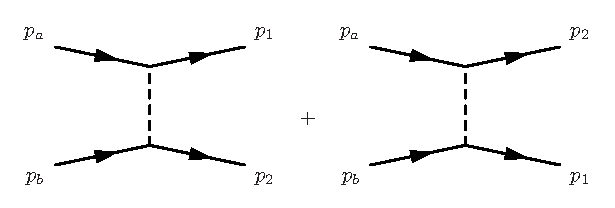
\includegraphics{\feynmfdirectory/01NNtoNNeq/NNtoNN.eps}
\nonumber\\
\label{eqn:scYSmtrxFeynmDiag}
\end{eqnarray}
%----------------------------------------
The final expression is written in terms of two Feynman diagrams
which correspond respectively to the two terms in Eq. (\ref{eqn:scYSelem}).
These diagrams are abbreviated a bit for a technical reason of the drawing.
A fully drawn diagram may look like the following figure.
\begin{figure}[h]
\vspace*{35mm}
%        positive in these values mean,  voffset: upward   hoffset: rightward
\special{psfile="\feynmfdirectory/02NNtoNNbig/NNtoNNtrim.eps" hscale=70 vscale=70 voffset=-0 hoffset=100}
\caption{Fully drawn Feynman diagram for the first term in Eq. (\ref{eqn:scYSmtrxFeynmDiag})}
\label{fig:scalarYNN2NNFeynm}
\end{figure}
Arrows on external lines indicate flows of conserved quantum numbers associated with
particles like baryon number, flavor and so on. In the current case, it is the electric charge
which is conserved in the Lagrangian density (\ref{eqn:sclYkwLagDens}) as is stated above
Eq. (\ref{eqn:scYelchrg}).
In many situations, we draw a diagram like Fig. \ref{fig:scalarYNN2NNFeynm} without
momentum arrows to represent the two diagrams in Eq. (\ref{eqn:scYSmtrxFeynmDiag}).


The correspondence between diagrams and equations are ensured by obeying
the so called Feynman rule described as follows:

\begin{enumerate}
\item For each external lines, associate a factor $1/\sqrt{(2\pi)^3}$.

\item To each vertex, associate a factor
\begin{eqnarray}
(-ig) (2\pi)^4 \delta^4(\sum_{in} p_{in})\,,
\end{eqnarray}
where $p_{in}$ denotes a momentum flowing into the vertex and the sum is taken
over all momenta connected to the vertex. Momenta flowing out from the vertex get
a minus sign. For the upper vertex in Fig. (\ref{fig:scalarYNN2NNFeynm}), for instance,
we read $\sum_{in} p_{in} = p_a - k - p_1$.

\item For each internal broken line, corresponding to a $\psi$ particle with momentum $k$,
write a factor of
\begin{eqnarray}
\int \frac{d^4 k}{(2\pi)^4} \frac{i}{k^2 - m^2 + i\epsilon}
\end{eqnarray}
When the internal line is solid, corresponding to a $\psi$ particle, write the same factor
with $m$ replaced by the nucleon mass $M$.
\end{enumerate}

The scattering amplitude $T_{fi} = \bra f \braend T \ketend i \ket$ 
in Eq. (\ref{eqn:Smatrix_and_T}) is now
written as
\begin{eqnarray}
T_{fi}
&=&
\frac{(-i g)^2}{(2\pi)^6} 
\left\{
\frac{1}{(p_1 - p_a)^2 - m^2}
+
\frac{1}{(p_2 - p_a)^2 - m^2}
\right\}
\nonumber\\
&=&
\frac{(-i g)^2}{(2\pi)^6} 
\left(
\frac{1}{t - m^2}
+
\frac{1}{u - m^2}
\right)
\end{eqnarray}
Finally, from Eq. (\ref{eqn:2to2cs}), we write the scattering cross section as
\begin{eqnarray}
\frac{d \sigma}{dt}
&=&
\frac{g^4}{16\pi \lambda(s, m_N^2,m_N^2)}
\left(
\frac{1}{t - m^2} + \frac{1}{u - m^2}
\right)^2
\end{eqnarray}

\bigskip

\stepcounter{exercise}
Exercise\theexercise:
Examine the kinematical regions for $t$ and $u$ in this scattering.

\bigskip

An enhancement of the cross section at small $|t|$ follows from the mass pole
of the exchanged pion. We also understand an enhancement at small $|u|$ is
a consequence of  the $t$-channel enhancement and the indistinguishability of
the two nucleons in the final state.


%----------------------------------------
\begin{comment}
Integral expression of the scattering matrix element in Eq. (\ref{eqn:scYSelem}) 
is written in terms of the Feynman diagram as
\begin{figure}[h]
\vspace*{30mm}
%        positive in these values mean,  voffset: upward   hoffset: rightward
\special{psfile="\feynmfdirectory/01NNtoNNeq/NNtoNN.eps" hscale=70 vscale=70 voffset=30 hoffset=70}
%\caption{Feynman diagram}
\label{fig:scalarYNN2NNinEq}
\end{figure}


&&
\unitlength=1mm  %<<<---------------------------------------------- scale
\parbox{40mm}
{
\begin{fmffile}{NNbyPi1}
	\begin{fmfgraph*}(40,20)
			\fmfleft{i1,i2}
			\fmfright{o1,o2} 
			%\fmfv{label=$p_b$, label.angle=90}{i1}
			\fmflabel{$p_b$}{i1}
			\fmflabel{$p_a$}{i2}
			%\fmfv{label=$p_a$, label.angle=270}{i2}
			\fmflabel{$p_2$}{o1}
			\fmflabel{$p_1$}{o2}
			\fmf{fermion,tension=2}{i1,v1,o1}
			\fmf{fermion,tension=2}{i2,v2,o2}
			\fmf{dashes}{v1,v2}
			%\fmflabel{$-ig(2\pi)^4 \delta^4(\sum_{in} p_{in})$}{v1}
			%\fmflabel{$-ig(2\pi)^4 \delta^4(\sum_{in} p_{in})$}{v2}
	\end{fmfgraph*}
\end{fmffile}
}
\hspace{3mm}
+
\hspace{3mm}
\parbox{40mm}
{
\begin{fmffile}{NNbyPi2}
	\begin{fmfgraph*}(40,20)
			\fmfleft{i1,i2}
			\fmfright{o1,o2} 
			\fmflabel{$p_b$}{i1}
			\fmflabel{$p_a$}{i2}
			\fmflabel{$p_1$}{o1}
			\fmflabel{$p_2$}{o2}
			\fmf{fermion,tension=2}{i1,v1,o1}
			\fmf{fermion,tension=2}{i2,v2,o2}
			\fmf{dashes}{v1,v2}
	\end{fmfgraph*}
\end{fmffile}
}
\end{comment}
%----------------------------------------

\bigskip
%=================================================================
\noindent
\underline{$N\overline{N} \to N\overline{N}$ amplitude}

\bigskip

Initial and final states:
\begin{eqnarray}
\begin{array}{l}
\ketend i \ket
=
b^\dagger(\bld{p}_a) c^\dagger(\bld{p}_b) \ketend 0 \ket
\rightdef
\ketend N(\bld{p}_a) \overline{N}(\bld{b}_b )\ket
\\
\ketend f \ket
=
b^\dagger(\bld{p}_1) c^\dagger(\bld{p}_2) \ketend 0 \ket
\rightdef
\ketend N(\bld{p}_1) \overline{N}(\bld{p}_2) \ket
\end{array}
\label{eqn:scYNNbarNNbarinit}
\end{eqnarray}
Since there are four nucleons in the initial and final states, we need at least 
four $\psi$ fields from interaction Hamiltonians and all $\phi$ fields should
be contracted out. Thus, S-matrix elements to the lowest order is written 
again as Eq. (\ref{eqn:scYS2ndord}). Evaluating sandwich factor as before,
we get
\begin{eqnarray}
\bra f \braend S - 1 \ketend i \ket
&\stackrel{(2)}{=}&
%\nonumber\\
%&&
\parbox{80mm}{
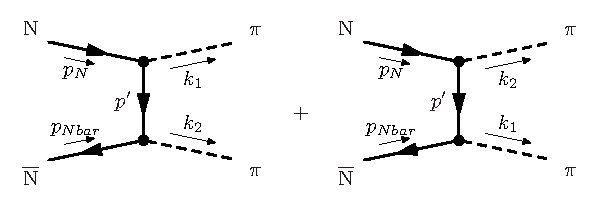
\includegraphics{\feynmfdirectory/03NNbar2NNbar/Smtrx2trim.eps}
}
\nonumber\\
\label{eqn:scYSmtrxFeynmDiag}
\end{eqnarray}
It reads
\begin{eqnarray}
T_{fi}
&=&
\frac{(-i g)^2}{(2\pi)^6} 
\left\{
\frac{1}{(p_a - p_1)^2 - m^2 \cancel{+ i\epsilon}}
+
\frac{1}{(p_a + p_b)^2 - m^2 + i\epsilon}
\right\}
\nonumber\\
&=&
\frac{(-i g)^2}{(2\pi)^6} 
\left(
\frac{1}{t - m^2}
+
\frac{1}{s - m^2 + i\epsilon}
\right)
\label{eqn:scYNNbar}
\end{eqnarray}
Cross section is obtained by adopting Eq. (\ref{eqn:2to2cs}) as before.
We omit $i \epsilon$ in the first term in Eq. (\ref{eqn:scYNNbar}) since
$t < 0$. In the second term, however, $s = m^2$ may occur when
$m > 2M$. This is why we remained $i \epsilon$ in the second term.
However, in this case, correction of the pion propagator due to higher
order terms with nucleon loops will bring a finite imaginary part into the
denominator of the propagator. Nevertheless, for the lowest order
tree diagram, we keep the $i \epsilon$ term.

\bigskip

\verb/-----------.-----------.-----------.-----------.-----------/\\
\vspace{-3mm}
{\small
\begin{center}
Addendum: Derivation of Eq. (\ref{eqn:scYSmtrxFeynmDiag})
\end{center}

It is still instructive to show the derivation of Eq. (\ref{eqn:scYSmtrxFeynmDiag}).
To evaluate Eq. (\ref{eqn:scYS2ndord}), we write
\begin{eqnarray}
\psi(x) = b(x) + c^\dagger(x)\,,
\hspace{3mm}
\psi^\dagger(x) = b^\dagger(x) + c(x)\,,
\end{eqnarray}
referring the form in Eq. (\ref{eqn:scYfields}).
In the following, we will include in our consideration the case that $\psi$ is fermion obeying
anti-commutation relationships instead of commutation ones in Eq. (\ref{eqn:complscalarcancomm}).
Considering the initial and final states in Eq. (\ref{eqn:scYNNbarNNbarinit}),
we need to remain terms $\sim b^\dagger c^\dagger bc$ in the sandwich of 
the normal order product in Eq. (\ref{eqn:scYS2ndord}). Since there are two
$\psi^\dagger$'s and two $\psi$'s, we have four ways to pick up necessary terms.
Keeping only relevant terms, we write
\begin{eqnarray}
\psi^\dagger(x_1) \psi(x_1) \psi^\dagger (x_2) \psi(x_2)
&=& 
\begin{array}{c}
b^\dagger(x_1) b(x_1) c(x_2) c^\dagger(x_2)
\\
+
\\
c(x_1) c^\dagger(x_1) b^\dagger(x_2) b(x_2)
\end{array}
+
\begin{array}{c}
b^\dagger(x_1) c^\dagger(x_1) c(x_2) b(x_2)
\\
+
\\
c(x_1) b(x_1) b^\dagger(x_2) c^\dagger(x_2)
\end{array}
%\nonumber\\
%&&
+ \mbox{irrelevant terms}
\nonumber
\end{eqnarray}
Inside the normal order product, terms with creation operators goes to the left.
When the fields are fermionic, an exchange of fields brings a minus sign. 
Omitting irrelevant terms, we write,
\begin{eqnarray}
\normalprod{\psi^\dagger(x_1) \psi(x_1) \psi^\dagger (x_2) \psi(x_2)}
&=& 
\left(
\begin{array}{c}
b^\dagger(x_1) c^\dagger(x_2) b(x_1) c(x_2) 
\\
+
\\
b^\dagger(x_2) c^\dagger(x_1) b(x_2) c(x_1)   
\end{array}
\right)
\pm
\left(
\begin{array}{c}
b^\dagger(x_1) c^\dagger(x_1) b(x_2) c(x_2)
\\
+
\\
b^\dagger(x_2) c^\dagger(x_2) b(x_1)  c(x_1)
\end{array}
\right)
\,,
\nonumber
\end{eqnarray}
where $+$ sign is taken for our bosonic nucleons and
$-$ is taken when nucleons are fermions.
Now we take the sandwich of this object between the initial and final states and
put it in Eq. (\ref{eqn:scYS2ndord}). There are integrations over $x_1$ and $x_2$
and their names can be exchanged:
\begin{eqnarray}
&&\int d^4x_1 d^4x_2
\bra f \braend
\normalprod{\psi^\dagger(x_1) \psi(x_1) \psi^\dagger (x_2) \psi(x_2)}
\ketend i \ket
\nonumber\\
&&=
2 \int d^4x_1 d^4x_2
\bra f \braend
b^\dagger(x_1) c^\dagger(x_2) b(x_1) c(x_2) 
\pm
b^\dagger(x_1) c^\dagger(x_1) b(x_2) c(x_2)
\ketend i \ket
\nonumber
\end{eqnarray}
Now we expand fields in the momentum space.
Considering assignments of momenta in the initial and final states,
we assign names of momentum variables accordingly:
\begin{eqnarray}
&&
\bra 0 \braend
c(\bld{p}_2) b(\bld{p}_1)
\left\{
b^\dagger(x_1) c^\dagger(x_2) b(x_1) c(x_2) 
\pm
b^\dagger(x_1) c^\dagger(x_1) b(x_2) c(x_2)
\right\}
b(\bld{p}_a) c(\bld{p}_b) 
\ketend 0 \ket
\nonumber\\
&&
\hspace{25mm}
p_1'
\hspace{5mm}
p_2'
\hspace{5mm}
p_a'
\hspace{5mm}
p_b'
\hspace{8mm}
p_1'
\hspace{5mm}
p_2'
\hspace{5mm}
p_a'
\hspace{5mm}
p_b'
\hspace{5mm}
\nonumber
\end{eqnarray}
The whole of Eq. (\ref{eqn:scYS2ndord}) reads
\begin{eqnarray}
\bra f \braend S - 1 \ketend i \ket
&=&
(-ig)^2 \int
\frac{d^3 \bld{p}_1' d^3 \bld{p}_2'}{(2\pi)^3 4p_1^{0'}p_2^{0'}}
\frac{d^3 \bld{p}_a' d^3 \bld{p}_b'}{(2\pi)^3 4p_a^{0'}p_b^{0'}}
\frac{d^4 k}{(2\pi)^4} \frac{i}{k^2 - m^2 + i\epsilon}
d^4x_1 d^4x_2
\nonumber\\
&&
\bra 0 \braend
c(\bld{p}_2) b(\bld{p}_1)
\left(
b^\dagger(\bld{p}_1') c^\dagger(\bld{p}_2') b(\bld{p}_a') c(\bld{p}_b')
\right)
b(\bld{p}_a) c(\bld{p}_b) 
\ketend 0 \ket
\nonumber\\
&&
\left\{
e^{i(p_1' - p_a' - k)x_1} e^{i(p_2' - p_b' + k)x_2} 
\pm
e^{i(p_1' + p_2' - k)x_1} e^{-i(p_a' + p_b' - k)x_2} 
\right\}
\nonumber\\
&=&
\frac{(-ig)^2}{(2\pi)^6} i (2\pi)^4 \delta^4(P_f - P_i)
%\nonumber\\
%&&
\int
\frac{d^4 k}{k^2 - m^2 + i\epsilon}
\left\{
\delta^4 (p_1 - p_a - k)
\pm
\delta^4 (p_a + p_b - k)
\right\}
\nonumber
\end{eqnarray}
thus recovers Eq. (\ref{eqn:scYSmtrxFeynmDiag})
as the bosonic case.
}\\
\verb/-----------.-----------.-----------.-----------.-----------/\\

\bigskip
%=================================================================
\noindent
\underline{$N\overline{N} \to \pi \pi$ amplitude}

\bigskip

Initial and final states:
\begin{eqnarray}
\begin{array}{l}
\ketend i \ket
=
b^\dagger(\bld{p}_a) c^\dagger(\bld{p}_b) \ketend 0 \ket
\rightdef
\ketend N(\bld{p}_a) \overline{N}(\bld{b}_b )\ket
\\
\ketend f \ket
=
a^\dagger(\bld{p}_1) a^\dagger(\bld{p}_2) \ketend 0 \ket
\rightdef
\ketend \pi(\bld{p}_1) \pi (\bld{p}_2) \ket
\end{array}
\label{eqn:scYNNbarPiPiinit}
\end{eqnarray}
This time we should go back to the first equation in Eq. (\ref{eqn:scYS2ndord})
for picking up
one $b$ from a $\psi$, one $c$ from a $\psi^\dagger$ and two $a^\dagger$'s from 
two $\phi$'s in the T-product. The remaining pair of $\psi$ and $\psi^\dagger$ are
contracted to give a propagator. The Wick's theorem in this time reads
\begin{eqnarray}
&&
T[
\psi^\dagger(x_1) \psi(x_1) \phi(x_1)
\psi^\dagger(x_2) \psi(x_2) \phi(x_2)
]
\nonumber\\
&&
= 
\bra 0 \braend T[]
\end{eqnarray}







